\hyphenation{a-no-ny-mi-ty}

\chapter{Background and Literature Review} \label{chap:sota}

\section*{}

This chapter will dive deep into previously done work related to this project. First, a Background is provided for the reader to have context on some relevant work and information that precedes the findings present in the following sections. Second, since the goal is to develop a complete application, there will be an analysis of the specific problems and how they have been solved in the literature. Then, there will be a comparison between a similar work and similar existing applications.

\section{Background}

Since this project is intended for general use, the easiest and most common client available to users is the web client, also known as a web browser. In the early stages of the web, the applications followed a server-client architecture where the client had little to no work: it just rendered some previously compiled HTML and CSS on the page, and the user made the interaction with the server through HTML forms. Later on, JavaScript usage increased, and the pages started to be a bit more dynamic \cite{ShklarRosen09}. Still, it wasn't until more performant and portable devices such as the iPhone were available to the public that web applications started to tilt their focus to the client-side. 

More recently, we start to see \say{Single Page Applications}, which harness the client-side JavaScript capabilities to simulate legacy web interactions such as changing to another page or view without actually reloading the page, trading client-side work for network load \cite{Lugo-Cordero2015} \cite{Derezinska2020} \cite{Mesbah2007} \cite{Mesbah2007a}. In this architecture, there still exists a server and clients (the web browsers). However, the server usually serves a REST API (Representational State Transfer Application Programming Interface) and a bare-bones HTML document, which serves as a base for the clients to render the rest of the document with JS, based on API calls results. There is also a mixed option: The server handles some logic, usually related to session management or localization, and responds with an HTML document that already has some information to prevent the client-side from taking too much time on work done for every request. On the web, some frameworks allow this more recent architecture, such as React\footnote{https://reactjs.org/}, Vue\footnote{https://vuejs.org/} and Angular\footnote{https://angular.io/}.

\begin{figure}[t]
    \begin{center}
      \leavevmode
      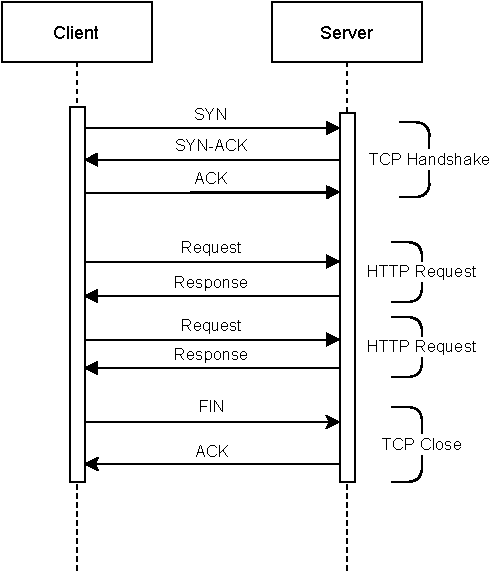
\includegraphics[width=0.6\textwidth]{http-protocol.pdf}
      \caption{HTTP protocol example interactions}
      \label{fig:http-protocol}
    \end{center}
  \end{figure}

Since the web uses the HTTP Protocol \cite{http1-1protocol} \cite{http2protocol}, it is quite hard to achieve real-time behavior with good performance, due to the protocol's design \cite{Spero1994}. As shown in Figure \ref{fig:http-protocol}, every data transfer starts with a request and ends with a response. It is therefore tied to this two-step process, which limits its potential. 

To allow a more performant way of data transmission between client and server, similar to the well-known data sockets available in Operating Systems used for bi-directional data transfer in real-time, there exist Web Sockets \cite{websocket-protocol} which serve the same purpose and allow Web Applications to send real-time updates to the clients without them needing to request them, which would only be possible otherwise using techniques such as polling (i.e.,\ the client keeps asking the server for updates periodically), and even here, the client is actually asking for updates, only in fast succession.

When developing a Web Application, one of the most important aspects is User Experience (UX). It is even more relevant than User Interface (UI) because, even though they impact one another, an application with a good UI but poor UX is just a nice painting the users can look at and be amazed, but with no interaction whatsoever.

According to Tullis and Albert \cite{measuring-user-experience-tullis}, UX involves a user, that user's interaction with the interface, and the interest in observing or measuring their experience when using the interface. A more common concept is usability, which is usually considered to be the ability of the user to use the interface to execute a task successfully.

In order to have a good UX, an application cannot require too much thinking from the user, it should be intuitive \cite{Krug2013-ux}. The application should be self-explanatory and \say{nothing important should be more than two clicks away}. This involves link naming, placement, colors, and more, hence its connection to the UI.

Even though some things have specific rules (e.g.,\ links should be say{clickable} and look like it), others require further examination to understand how users are interacting with them. This is done manually in usability tests, where actual human users are recruited and product owners can see directly how they execute some requested action, and feedback is provided directly; or automatically, through UX metrics.

UX metrics can be of different types \cite{measuring-user-experience-tullis}: performance, usability, self-reported (i.e.,\ satisfaction/ease-of-use rating given by the user) and behavioral/phsycological.

Performance metrics include measuring task success ratios, timing tasks (i.e.,\ how much time does it take for a user to do something) and error collection. Usability metrics rely on the users reporting of issues they encounter when using the application. Self-reported metrics are small questionnaires filled in by users, usually at the end of an interaction/session, which give a more complete information about what the experience felt like for the user. Behavioral/Psychological metrics take advantage of sensors in order to measure reactions via eye-tracking and heart rate monitoring, for example.

As with any software application, there must some kind of tests in place, in order to guarantee a minimal quality standard. In the interface domain, tests rely more on simulation user actions, such as clicking on components, inputting text, submitting forms, etc., and asserting the results of those actions on the webpage. To develop unit-tests following this model, there are libraries such as Testing Library\footnote{https://testing-library.com/} which allows for asserting page changes in multiple frameworks --- such as React, Vue or Angular, mentioned above, and more. For more complex tests, relying on the full application --- including the server --- which simulate the complete interaction of a user with the application, also called end-to-end tests, there are alternatives like Selenium\footnote{https://www.selenium.dev/} and Puppeteer\footnote{https://pptr.dev/}, which simulate actions on an actual browser, not only on a simulated webpage, thus allowing that browser to dynamically change based on the server behavior and on interaction with other clients, rendering it very useful when testing multi-user applications.

\section{Offline Availability}\label{sec:offline-avail-sota}

As stated in \cite{Mark2008}, even though people complete interrupted tasks in less time with no quality drop, interruptions make users work faster to compensate for it, increasing stress and frustration. The lack of offline interaction would force users to interrupt their task of inputting the desired information. That would increase stress when adding it later once they connect again, as they would try to do it fast while that information still has relevance. Indeed, a real-world application was tested in both scenarios --- with offline mode and without it --- for which the basic version obtained a user satisfaction score of 66.5. In contrast, the offline-tolerant version had a score of 95.5 out of 100 points, proving that having an offline mode improves the user experience in a web application substantially \cite{Marco2015}. 

Marco \cite{Marco2013} exposes the interrupted internet connectivity problem applied to e-learning applications. It proposes creating a modeling tool to create interruption-resilient web applications by defining the possible operations and how they should behave in case of interruption. This model is presented later \cite{Abertos-Marco2017}, proposing the Offline Model, which defines a taxonomy for interruptions on web applications. It further analyzes some properties of web applications in the presence of interruptions, such as scheme and offline support, which depend on the application and the task being performed within it.

Marco further specifies rules regarding adapting basic web applications into offline-tolerant ones \cite{Marco2015}. On the \textit{Application Domain Level}, the data model of the application should not be modified to support as many applications as possible. Regarding the \textit{Hypertext Level}, the navigation on the application could be slightly modified or adapted, regarding pages within the web application, depending on the connectivity status. On the \textit{Presentation Level}, the user interface (UI) should be adapted according to policies specific to each page element as the interaction with those elements would change depending on the connectivity status.

Therefore, it is necessary to establish which components of the web application will be available in offline mode and how.
To specify the navigation, they propose the notation presented by Albertos et al.\ \cite{Penichet2013}, representing the web pages as nodes, with edges meaning navigation within the web application. Each node has attributes referring to policies about the behavior of the components in offline mode and the mechanism to create the local copy. To specify the interface behavior in offline mode, the following policies are described:

\begin{itemize}
    \item \textbf{Hide}: The element should be hidden, preventing user interaction
    \item \textbf{Disable}: The element should be shown, but interaction should not be possible
    \item \textbf{Save}: Save elements locally so that they can be accessed in offline mode (such as images or text documents)
    \item \textbf{Update}: For elements that can be interacted with when in offline mode, they should be updated --- synchronized --- when connectivity is regained
\end{itemize}

Yang \cite{Yang2000} presents a mechanism to support offline collaborative work in a web application. Due to the publication's age, most of the used tools are now obsolete, but the general ideas still apply. It proposes the existence of local storage to every client so that operations done in offline mode are kept. Then, once the user comes back online, the work saved in the local storage is synchronized with the online storage, where conflict-resolution algorithms take place in order to minimize said conflicts.

Kleppmann, Wiggins, Hardenberg et al.\ \cite{Kleppmann2019} propose ideals for local-first software, being the idea that the data on users' local machines is the primary when compared to servers, not the other way around, as it often happens in web applications:

\begin{enumerate}
    \item \textbf{\say{No spinners} / No loading}: Data is changed locally, and synchronization occurs quietly in the background;
    \begin{itemize}
        \item A workaround pattern is mentioned --- Optimistic UI --- which consists of showing the changes immediately, while sending them to the server, which would need to be reverted in case of error, for example
    \end{itemize}
    \item \textbf{Multi-device support}: Users should be able to work everywhere;
    \item \textbf{Optional network}: Since local-first applications store the primary copy of their data in each device’s local file system, the user can read and write this data anytime, even while offline. It is then synchronized with other devices sometime later, when a network connection is available;
    \item \textbf{Seamless Collaboration}: Real-Time collaboration should be possible with conflict resolution when necessary;
    \item \textbf{Data Forever}: The data is independent of the company or service provider, since it is stored locally. It should therefore last forever;
    \item \textbf{Secure and Private by default}: By having the data on each user's device locally, database tampering is not as harmful, as you'll have many backed up replicas. Moreover, by using end-to-end encryption, the server can only save encrypted data, thus making it private, as it can only be decrypted by the users who are allowed to do so;
    \item \textbf{Ownership}: The user owns the data, the provider cannot block the access in any form since the data is local.
\end{enumerate}

It further compares multiple applications in the way they handle the local-first ideals, such as Files and Email attachments, or Google Docs\footnote{https://www.google.com/docs/about/} as well as technologies to implement said ideals, such as Web Applications, Mobile Applications, CouchDB\footnote{https://couchdb.apache.org} --- a multi-master database that allows each node to mutate the database and synchronize the changes with other nodes, meant to run on servers --- and PouchDB\footnote{https://pouchdb.com/} --- with the same goal of CouchDB, but meant to run on the end-user devices.

It also mentions CRDT (Conflict-Free Replicated Data Types) as a foundational technology to achieve the local-first ideals. As explained in the next section,  CRDT are general-purpose data structures similar to the common lists and maps but built for multi-user environments from the beginning. CRDT merge changes from multiple users when possible; however, it does not handle changes to the same element in the structure. In that case, it keeps track of the conflicts for the application to deal with them, allowing for custom conflict resolution techniques. CRDT are generic enough to synchronize over any communication connection like server, peer-to-peer networks, Bluetooth, and others. The paper further presents \textit{Automerge}\footnote{https://github.com/automerge/automerge} as a JavaScript (JS) CRDT implementation.

Furthermore, the authors built some prototypes using Electron, JavaScript, and React using CRDT to verify that its usage was viable to build local-first software for the web and desktop applications. The main conclusions were that CRDT worked reliably while integrating easily with the other tools and seamlessly merging data. Also, they verified that the user experience was splendid, as it allowed for offline work and sync when possible, giving the feeling of \say{data ownership} to the user. Finally, they state that this technology combines well with Functional Reactive Programming (FRP), a paradigm that renders the view based on a function that receives data. If the data changes, it \say{reacts} and redraws. A popular framework enabling this paradigm is React, but there are others such as Vue or Flutter. With such a tool, by syncing the data with a CRDT and reacting to UI changes, a real-time experience is achieved.

Finally, it added that CRDT might have a performance problem if used to save many changes (since they essentially save all the history). That is something that must be taken into account when using that technology and designing the system.

Zawirski, Preguiça, Duarte et al.\ \cite{Zawirski2015} proposes a way of supporting many client-side applications by sharing a database of objects that they can read and update under a convergent causal consistency model, with support for application-specific conflict resolution. It relies on fast local writes, and possibly stale data reads to achieve better speeds. It allows updates to thousands of clients using only three data centers, leveraging client buffering and controlled staleness, absorbing the cost of scalability, availability, and consistency.

Kao, Lin, Yang et al.\ \cite{Kao2012} proposes a system to allow mobile applications to run in a web container, joining the benefits of both: being able to run offline and cross-platform.

In order to make it possible for users to work while they are not connected to the internet, there must be a way of storing their actions locally so that they can be synchronized when they regain internet connectivity. Currently, HTML5 exposes multiple local storage APIs, which can be used for this effect.

Liu \cite{Liu2014} discusses multiple web client storage technologies, comparing their advantages and disadvantages:
\begin{itemize}
    \item \textbf{Cookies}: Small piece of data that is included in every HTTP request (limit of 4 KB per cookie \cite{cookies-rfc}). They can be managed by the server as well as the client and are mostly used to keep state in between HTTP requests, for use cases such as user sessions or keeping track of some user activity. They are very popular and widely used, but at the same time they have little capacity and can be insecure, due to their presence in the HTTP communication with the server \cite{Velagapudi2019} \cite{Kwon2020};
    \item \textbf{localStorage}: Can be used to implement cross-page communication (in the same domain) by storing data and having the web application listen for storage events, all pages of the same domain will have the updated data in the respective section of \textit{localStorage}. It can be faster than cookies since no interaction with the server is needed.
    The data is stored in key-value pairs and is partitioned by domain, with no risk of inter-domain data corruption. It can be read and modified using JavaScript and all values are strings.
    \item \textbf{sessionStorage}: Works in the exact same way as \textit{localStorage}, but the data only lasts until the browser is closed, i.e.,\ the session;
    \item \textbf{UserData}: Older technology, specific to Internet Explorer, and has since been deprecated, it had only 128 KB of capacity;
    \item \textbf{Web SQL Databases}: Uses a table-structured format to store the local data. In Google Chrome, it uses the SQLite DB. The interactions are made as it were a normal SQL database running, by using the $executeSql()$ or $transaction()$ APIs. It is not supported by all browsers nor is it part of W3C standard\footnote{https://www.w3.org/TR/webdatabase/};
    \item \textbf{Indexed Database}: Uses a NoSQL DB to store the data. Event-based so it is asynchronous by default. It might be helpful to use a Promise-based wrapper \cite{promises-js-mdn} such as idb\footnote{https://www.npmjs.com/package/idb}.
\end{itemize}
Liu further concludes that \textit{localStorage} is the most compatible among web browsers. In summary, for session id tracking or for small data storage, one should use \textit{Cookies}; up to 5 MB, \textit{localStorage} delivers a solution across all common browsers\footnote{https://www.w3.org/TR/webstorage/}; for more space, \textbf{Indexed Database} is recommended.

Jemel and Serhrouchni \cite{Jemel2014} presents some vulnerabilities that can arise from using the HTML5 Local Storage API as is. It also introduces a way of securing data stored using the local storage API, based on the user, not only the domain the data belongs to.


\section{Conflict resolution}\label{sec:conflict-res-sota}

Conflict resolution is a problem that has been studied extensively in the literature, with publications dating as far back as 1986 \cite{Greif1986}. Still, it was not until 1989 that the first algorithm was proposed to deal with this problem by Ellis and Gibbs \cite{Ellis1989}.

In that paper, they define groupware systems as multi-user (i.e.,\ composed of two or more users) computer systems that allow development on a common task, providing an interface to a shared environment. They propose an algorithm to solve the groupware real-time concurrency problem called \textbf{Operational Transformation (OT)} which allows concurrent editing without the need for locks, increasing responsiveness. \textit{Response time} is defined as the time required for the user's action to be reflected on their screen. \textit{Notification time} is defined as the time required for the user's action to be propagated to all other participants.

Real-time groupware systems have the following characteristics:

\begin{itemize}
    \item \textbf{Highly interactive}: Short response times;
    \item \textbf{Real-time}: Notification times should be close to the response times;
    \item \textbf{Distributed}: They should work even if the participants are connected in different machines and networks on the internet;
    \item \textbf{Volatile}: Participants may enter and leave the session at any time;
    \item \textbf{\textit{Ad Hoc}}: Participants don't follow a script, it is therefore impossible to know what is the information they are trying to access beforehand;
    \item \textbf{Focused}: Generally users will be trying to access the same data, generating a high degree of access conflicts;
    \item \textbf{External Channel}: Participants are often connected among them via an external channel such as an audio or video communication tool;
\end{itemize}

A groupware system model is then defined as being formed by a set of sites and operators. Sites consist of a site process (i.e.,\ a user's unique session), a site object (i.e.,\ the data being read and modified), and a unique site identifier. Operators are the set of operations available for users to apply to the site objects. The goal is to maintain consistency among all the site objects at all times. The site process performs three kinds of activities: \textbf{operation generation}, where the user generates an operation to be applied to the site objects. The site will then encapsulate the action in an operation request to be broadcasted to all other sites; \textbf{operation reception}, where an operation is received from another site; \textbf{operation execution}, where an operation is executed on the local site object. The model further assumes that the number of sites is constant, messages are received exactly once, without error, and that it is impossible to execute an action before it is generated.

The paper further specifies the following definitions regarding the groupware system:

\begin{itemize}
    \item Given two operations $a$ and $b$, generated at sites 1 and 2, respectively, $a$ precedes $b$ iff:
    \begin{itemize}
        \item $a = b$ and the generation of $a$ happened before the generation of $b$, or
        \item $a \neq b$ and the execution of $a$ on site 2 happened before the generation of $b$;
    \end{itemize}
    \item The \textbf{Precedence Property} states that if an operation $a$ precedes another operation $b$, then at every site the execution of $a$ happens before the execution of $b$;
    \item A groupware session is \textbf{quiescent} iff all generated operations have been executed at all sites;
    \item The \textbf{Convergent Property} states that site objects are identical at all sites at quiescence;
    \item A groupware system is \textit{correct} iff the \textbf{Convergent Property} and the \textbf{Precedence Property} are always satisfied.
\end{itemize}

The proposed algorithm uses four auxiliary data structures: State vector, Request, Request Queue, Request Log and a predefined, semantics-based matrix of transformations. 

\textit{State Vectors} are based on the partial ordering definition in \cite{Lamport1978} and the concept of vector clocks in \cite{Liskov1986} and \cite{Fidge1988}, stores the amount of operations done per site, i.e.,\ the $i$'th component of the vector represents how many operations from site $i$ have been executed in the current site. It is therefore possible to compare two state vectors $s_i$ and $s_j$:
\begin{itemize}
    \item $s_i = s_j$ if each component of $s_i$ is equal to the corresponding component in $s_j$;
    \item $s_i < s_j$ if each component of $s_i$ is less than equal to the corresponding component in $s_j$ and at least one component of $s_i$ is less than the corresponding component in $s_j$;
    \item $s_i > s_j$ if at least one component of $s_i$ is greater than the corresponding component in $s_j$;
\end{itemize}

\textit{Requests} are tuples in the form $<i,s,o,p>$ where $i$ is the originating site's identifier, $s$ the originating site's state vector, $o$ is the operation and $p$ is the priority associated with $o$.
From the request state vector, a site can determine if the operation to execute can be executed immediately, or wait for needed updates from other sites, enforcing the precedence property. The \textit{Request Queue} is a list of requests pending execution. Even thought the term \say{queue} is used, it does not imply first-in-first-out order. The \textit{Request Log} stores at site $i$ the executed requests at that site, in insertion order.

The Transformation Matrix defines, for every operation type pair, a function $T$ that transforms operations so that given two operations $o_i$ and $o_j$, with priorities $p_i$ and $p_j$, instances of operators $O_u$ and $O_v$, respectively and
\begin{equation*}
    o'_j = T_{uv}(o_j, o_i, p_j, p_i)
\end{equation*}
\begin{equation*}
    o'_i = T_{vu}(o_i, o_j, p_i, p_j)
\end{equation*}
then $T$ is such that
\begin{equation*}
    o'_j \circ o_i = o'_i \circ o_j
\end{equation*}
where $\circ$ means composition of operations.

The algorithm has an initialization section, a generation section, a reception section, and an execution section.
In the initialization section, the site's log and request queue are set to empty, and the state vector is initialized with all values being 0 since no operations have been done. The next section specifies that whenever a local operation is received, a request is formed, and it is added to the local queue and broadcasted to other sites. In the receiving section, when a request is received, it is simply added to the request queue. Finally, the execution section specifies how to apply the operations, handling conflicts. First, it checks the request queue to retrieve any request (with state $s_j$) that can be executed, $s_i$ being the state in the local site $i$, and there are three possibilities:

\begin{enumerate}
    \item $s_j > s_i$: The request cannot be executed since there are changes done in site $j$ that were not executed yet at site $i$, therefore the request must be left in the queue for later execution;
    \item $s_j = s_i$: The two states are equal, therefore the request can be executed immediately without operation transformation
    \item $s_j < s_i$: The request can be executed, but the operation must be transformed, since site $i$ has executed requests that are preceded by request $j$, $r_j$. Site $i$'s log $L_i$ is examined for requests that were not accounted for by site $j$ (i.e.,\ the requests that were executed in $i$ but not on $j$ prior to the generation of $r_j$. Each such request is then used to transform $o_j$ in $o'_j$, according to the Transformation Matrix. $o'_j$ is then executed and the state vector is incremented.
\end{enumerate}

Some changes were later proposed to the state vector technique \cite{Landes2006} \cite{Almeida2008} to allow dynamic entries instead of a constant number of concurrent participants. Ellis and Gibbs \cite{Ellis1989} mentioned this in the OT definition and addressed it, noting that participants can enter and leave every time the system is quiescent since the Request Logs can be reset, and it should function as a checkpoint on each site.

Nichols, Curtis et al.\ \cite{Nichols1995} build another algorithm on top of the existing OT, presented in \cite{Ellis1989} that uses a server managing the collaboration, instead of being peer-to-peer like the former. This reduces the need for the request priority fields in the requests for tie-breaking since the server can use a different strategy such as a reputation system, which the next section will develop upon. By removing the need for multicasting, since the server orchestrates the process and the communication is done in server-client pairs only, there is no need for message reordering logic, since a message transport protocol such as TCP \cite{tcpprotocol} can be used instead, ensuring message delivery in the correct order before reaching the application layer, thus reducing the clients' workload.

Wang, Bu, and Chen \cite{Wang2002} propose a multi-version approach to resolving conflicts in a real-time multi-user graphic designing system. It is a \textbf{Compatible-Precedence} approach since, unlike a \textbf{Conflict-Precedence} approach where the objects are locked for resolution by users in case of conflict, in this case, the conflict resolution is made by the system. It proposes a classification of operations in one of two types: Non-Multi-version Operations (NMO) and Multi-version Operations (MO). The first are operations that, when in conflict, can be resolved by choosing one of them. The latter are better suited to be decided by the users; hence keeping both versions of the operation history is necessary.
To represent this model, it uses a left-subtree-child and right-subtree-sibling binary tree. The left-subtree represents the continuous conflict-resolved operations. Each node will have a right-child representing a conflicting operation, thus creating a different branch with its own history by adding left children to it. Finally, it proposes a set of algorithms to insert operations depending on their category --- NMO or MO --- and undo operations.

Citro, McGovern, and Ryan \cite{Citro2007} present an algorithm to handle both exclusive and non-exclusive conflicts. Exclusive conflicts are those in which operations leading to it neither can be realized at the same time nor can be executed in a specific order since the operations leading to the conflict overwrite each other, so it is impossible to define an order for them to execute maintaining the intention of both users. Non-Exclusive conflicts are those in which the operations can be realized simultaneously, being handled using conventional consistency management techniques such as operational transformation \cite{Ellis1989}.

The paper builds on top of existing techniques such as operational transformation and multi-versioning to handle both types of conflicts more effectively. Additionally, it does not suffer from a \say{partial intention} problem, since it allows delayed post-locking, based on the post-locking of objects technique proposed by Xue et al.\ \cite{Xue2001}. With this technique, users can fully express their intentions on the object, allowing for a more informed decision when manually resolving the conflict; it also does not require a group leader or other conflict resolution roles in order to resolve conflicts.

Over the years, more implementations were published, each with its own advantages and compromises, but for the sake of keeping the focus of this document in a more general view of existing alternatives, I redirect the reader to the OT Wikipedia article, which has a good summary table\footnote{https://en.wikipedia.org/wiki/Operational\_transformation\#OT\_control\_(integration)\_algorithms} of most of the alternatives and their characteristics. Additionally, Sun, Chengzheng provides a FAQ page\footnote{https://www3.ntu.edu.sg/scse/staff/czsun/projects/otfaq/\#\_Toc321146200}, serving as a knowledge base about the topic. This being a popular algorithm, many tools implement it and can be included in an application, such as TogetherJS\footnote{https://togetherjs.com}, based around what they call the hub: a server that everyone in the session connects to which echoes messages to all the participants using WebSockets, or ShareDB\footnote{https://github.com/share/sharedb}, a real-time database backend supporting OT. The default implementation of ShareDB is an in-memory, non-persistent database with no queries. It is possible, however, to create connectors for other databases and connectors are provided for MongoDB\footnote{https://www.mongodb.com/} and PostgreSQL\footnote{https://www.postgresql.org/}.

ShareDB is horizontally scalable using a publish and subscribe mechanism, making it relatively future-proof. Since it uses Express.js for the server, it is possible to use middleware to hook into the server pipeline and modify objects as they pass through ShareDB, adding flexibility.

Conflict-free Replicated Data Types (CRDT) are a different approach to the real-time coordination of inputs problem in a groupware system \cite{Shapiro2011}. They can be operation-based \cite{Letia2010} \cite{Baquero2014}, similar to OT, or state-based \cite{Baquero1999} \cite{Almeida2014}.

Operation-based CRDT are also called commutative replicated data types, or CmRDT. CmRDT replicas propagate state by transmitting only the update operation, similarly to OT. Replicas receive the updates and apply them locally. The operations are commutative. However, they are not necessarily idempotent. Therefore, the communications infrastructure must ensure that all operations on a replica are delivered to the other replicas, without duplication, but in any order.

State-based CRDT are called convergent replicated data types, or CvRDT. In contrast to CmRDT, CvRDT send their full local state to other replicas, where the states are merged by a function that must be commutative, associative, and idempotent. The merge function provides a join for any pair of replica states, so the set of all states forms a \textit{semilattice}. The update function must monotonically increase the internal state, according to the same partial order rules as the \textit{semilattice}. Kleppmann, Martin provides good presentations\footnote{https://www.infoq.com/presentations/crdt-distributed-consistency/}\footnote{https://gotocon.com/berlin-2016/presentations/show\_talk.jsp?oid=7910} on the CRDT topic. Similarly to OT, CRDT also has available libraries and tools to be used in applications. Riak\footnote{https://riak.com/introducing-riak-2-0/} is a distributed NoSQL key-value data store based on CRDT. Bet365 is an example of a large system using Riak\footnote{https://bet365techblog.com/riak-update}. Another example of CRDT implementation is Facebook's Apollo database\footnote{https://dzone.com/articles/facebook-announces-apollo-qcon}, showing that CRDT can be used at scale as well.

A third and more recent alternative to the conflict resolution problem is Differential Synchronization \cite{Fraser2009} \cite{Fraser-diff-sync-web}. It provides an alternative to OT, being a symmetrical algorithm, as it has nearly identical code in both client and server; state-based, thus not requiring a history of edits to be kept by clients; asynchronous, since it does not block user input while waiting for the response over the network; network resilient, convergent, suitable for any content for which semantic diff and patch algorithms exist; and highly scalable. A working example of this algorithm can be seen in MobWrite\footnote{https://code.google.com/archive/p/google-mobwrite/}.

As it can be noted, real-time applications usually apply a replicated architecture, where each client has its own replica, a user may directly edit its own version, realizing its effect immediately. The effects are then propagated to other clients.
Propagation can be operation-based \cite{Oster2006} \cite{Sun1998-ot} \cite{Sun1998} \cite{Weiss2009} or state-based \cite{Fraser2009}. Chengzheng, David, Agustina et al.\ \cite{Chengzheng2020} state that most real-time co-editors, including those based on OT and CRDT, have adopted the operation propagation approach for communication efficiency, among others. It continues by comparing both solutions. Firstly, CRDT solutions have significantly higher time and space complexities than OT solutions, as revealed in \cite{Sun2020}. Secondly, CRDT has a higher initialization cost since it needs to represent initial characters on the document, whereas OT's data structures start empty. This can have a big impact on session management and handling users that enter mid-session. Thirdly, OT does not have any additional time or space cost for non-concurrent operations. The operations buffer can be emptied with garbage collection --- as was previously mentioned, the system can reset some data structures every time it is quiescent. CRDT, on the other hand, will have similar time and space costs regardless of handling concurrent or sequential operations, as all operations will be applied in the internal object sequence, which can never be emptied unless the document itself is emptied. Finally, OT does not have any additional time or space cost for local operations, as they will never be concurrent with any operation in the Requests Log. CRDT, on the other hand, will have similar time and space costs regardless of handling local or remote operations, as all operations will be applied in the internal object sequence. The longer time the local operation processing takes, the less responsive the co-editor is to the local user. Herron \cite{Herron-ot-crdt} also compares OT to CRDT, looking at the implementation in a final application, revealing some examples and problems that can arise, such as the unwanted cursor movement.

In a more general way, Sun et al.\ \cite{Sun2012} present different types of conflict resolution in a creative editing system. The \textbf{preventive resolution} prohibits concurrent work on two same objects, avoiding conflicts altogether; \textbf{eliminative resolution} eliminates both operations when in conflict, eliminating the operations' history; \textbf{arbitrative resolution} elects one of the operations to be kept; \textbf{preservative resolution} keeps both options in different versions, so that the users can choose an alternative later; \textbf{creative resolution} produces a new operation, combining the two conflicting operations.

It further elaborates on the basic structure of a creative conflict resolution. There are three main components layered on top of each other. On the base, there is a conflict detector that simply detects if there are conflicts between operations. Next, there is a conflict synthesis component that creates the new operations based on the conflicts. Finally, there is the conflict management User Interface (UI), which is responsible for notifying users about conflicts and allowing them to select the desired conflict resolution strategy.

As important as the algorithm for solving conflicts themselves, the testing structure is also relevant. And in this scenario, creating relevant tests is more complex since they do not depend solely on a user's inputs and output assertions. Yu et al.\ \cite{Yu2007} propose a language to define test suites based on actors and a timeline of actions portrayed by them. This allows the developer to completely specify the actions of all the participants and their interactions in one place, asserting effects more clearly.

In summary, there are three alternatives for the conflict resolution in real-time problem: OT, CRDT, and Differential Synchronization, the latter having less development in the industry and not much production use. The two main strategies are operation synchronization (OT) and state synchronization (CvRDT). Operation synchronization broadcasts operations to be replicated among peers, whereas state synchronization broadcasts the state updates directly. These can be used for the automatic merge of conflicting operations, however, multi-versioning and creative resolution are techniques that can be applied for specific conflicts.

\section{Reputation System}\label{sec:rep-sys-sota}

There are multiple examples of how reputation can be used in multi-user systems and how it can affect group dynamics. Many refer to it as a solution to \say{Group Recommendations}, which are based in \textbf{trust} among participants, whereas others mention its ability to induce cooperation. Haveliwala \cite{Haveliwala2003} shows how the PageRank algorithm can be personalized so that each link among nodes has a different weight in order to express a dynamic preference among nodes. Andersen et al.\ \cite{Andersen2008} demonstrates multiple trust-based recommendation systems and how they comply with a set of relevant axioms. Most importantly, it shows how the aforementioned personalized PageRank (PPR) algorithm can be used to simulate a trust network among peers by linking users with differently weighted connections. The greater the weight, the more a user trusts another, and the most likely it is for the Random Walk algorithm to choose that \say{path of trust}. The latter also shows that PPR satisfies three out of five relevant axioms: \textbf{Symmetry}, \textbf{Positive Response}, \textbf{Transitivity}, but not Independence of Irrelevant Stuff and \textbf{Neighborhood Consensus}.
\begin{itemize}
    \item \textbf{Symmetry} --- Isomorphic graphs result in corresponding isomorphic recommendations (anonymity), and the system is also symmetric
    \item \textbf{Positive response} --- If a node’s recommendation is 0 and an edge is added to a + voter, then the former’s recommendation becomes +.
    \item \textbf{Transitivity} --- For any graph (N, E) and disjoint sets $ A, B, C \subseteq N $, for any source s, if s trusts A more than B, and s trusts B more than C, then s trusts A more than C.
    \item \textbf{Independence of Irrelevant Stuff (IIS)} --- A node’s recommendation is independent of agents not reachable from that node. Recommendations are also independent of edges leaving voters.
    \item \textbf{Neighborhood consensus} --- If a nonvoter’s neighbors unanimously vote +, then the recommendation of other nodes will remain unchanged if that node instead becomes a + voter.
\end{itemize}

Dellarocas \cite{Dellarocas2005-rep-mech} shows examples of how multiple platforms handle their user reputations mechanisms. It also states that reputation systems can prevent badly intended users and deter moral hazard by acting as sanctioning devices. If the community punishes users that behave poorly and if the punishment compensates the \say{cheating} profit, then the threat of public revelation of a user's cheating behavior is an incentive for users to cooperate instead. It further elaborates on the reputation dynamics of a multi-user application: 
\begin{itemize}
    \item \textbf{Initial Phase} --- Reputation effects begin to work immediately and in fact are strongest during the initial phase, as users try and work hard to build a reputation on themselves. Reputation effects may fail, however, when short-run users are “too cautious” when compared to the long-run ones and therefore update their beliefs too slowly in order for the long-run user to find it profitable to try to build a reputation;
    \item \textbf{Steady state} (or lack thereof) --- In their simplest form, reputation systems are characterized by an equilibrium in which the long-run user repeatedly executes the safe action, also known as the Stackelberg action, and the user's reputation converges to the Stackelberg type (always collaborating and no cheating).
\end{itemize}

These dynamics have important repercussions for reputation systems. Dellarocas goes on to say that if the entire feedback history of a user is made available to everyone and if a collaborator stays on the system long enough, once they establish an initial reputation for honesty, they will be tempted to cheat other users sometimes. In the long term, this behavior will lead to an eventual collapse of his reputation and, therefore, of cooperative behavior.

Bakos and Dellarocas \cite{Bakos2003} present a model for a reputation system that explores the ability of online reputation mechanisms to efficiently induce cooperation when compared to contractual arrangements relying on the threat of litigation. It concludes that the effectiveness of a reputation mechanism in inducing cooperative behavior depends on the frequency of transactions that are affected by this mechanism, reminding that a minimum degree of participation is required before reputation can induce a significant level of cooperation. After this threshold is reached, however, the power of reputation manifests itself, and high levels of cooperation can be supported.

Dellarocas \cite{Dellarocas2006-update-freq} concludes that reputation mechanisms can induce higher cooperation and efficiency if, instead of publishing updated ratings as soon as they are available, they only update a user's public reputation every $n$ transactions, meaning a summary statistic of a user's last ratings. In settings with noise, infrequent updating increases efficiency because it decreases the adverse consequence of artificial negative ratings. At the same time, however, infrequent updating increases a user's short-term gains from bad behavior and thus the minimum future punishment threat that can sustain cooperation.

Tests were made in order to understand the reputation issues for users \cite{Afonso2016}. These were made in Waze, a navigational driving assistant with crowd collaboration for road events. Even though this and zerozero.live are somewhat different, some parallelisms can be made, and some gathered information still applies. They concluded that it was hard for users to recognize where the information came from and if it was reliable at all. Furthermore, users did not care much about their reputation when submitting information (i.e.,\ if they heard about some road event, they would publish it without verifying it), maybe this is somewhat different from our use-case of sporting events, as users are either actually watching the game, or following it from a reliable source. Additionally, when users knew the source of data, they tended to trust people in their close circle (e.g., family and friends), and the main conclusion is that the app needed to convey the reputation of the source better to let the consumers know how much they can or should trust the source.

Resnick et al.\ \cite{Resnick2000} elaborate about reputation systems and their generic importance on the web. It is more geared towards e-commerce examples where people investigate the reputation before interacting with each other. It mentions three important properties reputation systems should have:
\begin{itemize}
    \item Long-lived entities that inspire an expectation of future interaction. If the entities are short-lived, their reputation matters little;
    \item Capture and distribution of feedback about current interactions (such information must be visible in the future);
    \item Use of feedback to guide trust decisions;
\end{itemize}
In the zerozero.live case, it might be hard to get expressive feedback from users regarding other users. Therefore, it is important to have some implicit voting in place. Additionally, users are more inclined to express feedback when they disagree than when they agree, which means that the lack of negative feedback must be considered positive feedback to balance the system. Besides, users won't see the reputation of other users beforehand in order to decide to interact or not, as they simply enter the event without knowing who is also there, so it is important that they can see the reputation, or a variant of it (i.e.,\ some relative reputation based on the current group of users) while they are at the event (e.g., showing it next to the user's name).

Melnikov, Lee, Rivera et al.\ \cite{Melnikov2018} present a dynamic interaction based reputation model (DIB-RM), which is further evaluated in \cite{Yashkina2020}. It presents a method to measure reputation as a function of user interaction frequency, also contemplating a reputation decay if the users stop contributing to the platform. 

The aforementioned method is also present in \cite{Daly2009}, where the authors present a way to harness the \say{wisdom of the crowds}, very much in line with what is required in zerozero.live, since there is no express authority during the event. It presents an example of a document sharing system and the approach to rank the documents based on the number of readers, the author's reputation, the time dynamics of reader consumption, and the time dynamics of documents contributed by the user. This last one manifests indirectly but is still relevant: it means that if a user has less-frequent readers on their documents, their reputation will decrease, so the contribution to the main document's reputation --- the one they are reading now --- will be smaller.
Reputation values scale between 0 and 1, and they stick to the following rules:
\begin{enumerate}
    \item Every time a user consumes a document from an author, the author gains reputation according to:
    \begin{equation} \label{eq:rep-increase}
        newRep = oldRep + (1 - oldRep) * repReward  
    \end{equation}
    $repReward$ is a constant between 0 and 1 and should consider the number of entities in the system. As the paper states: \say{If the number of expected consumers is in the order of hundreds or thousands, then an overly high value of $repReward$ will potentially cause popular content to quickly converge towards 1 making it difficult to differentiate between similarly popular content}.
    \item Every time a user consumes a document, the document gains \say{reputation} --- meaning popularity in this case --- according to the same formula of \ref{eq:rep-increase};
    \item In order to take time dynamics into account, reputation should decrease over time, so that a \say{rich-get-richer} paradigm can be avoided. This is achieved by the following equation (both for users and for documents):
    \begin{equation}
        newRep = oldRep * decayCoeff^k
    \end{equation}
    $decayCoeff$ represents how much the reputation will change, and $k$ is the amount of time units that have passed since the last reputation update, i.e.,\ for a time unit of \say{days}, $k$ will be 0 in the first 24h, 1 in the next day, 7 in a week, and so on. This decouples the algorithm from the logistics, since the algorithm can now run in a fixed frequency, independently of the time units, and every time it re-calculates, it will give an accurate value. However, if for example the time unit is \say{day}, and the algorithm updates every week only, there will be an offset of 6 days in which the value will be outdated.
    \item Users with higher reputation matter more when calculating the document reputation changes:
    \begin{equation}
        newRep = oldRep * repConsumer * B
    \end{equation}
    $B$ is a constant within [0, 1] representing to what extent the user reputation $repConsumer$ will influence the document's reputation.

    This system can be adapted and applied in zerozero.live if we map user inputs in an event as documents. However, we will be ranking users instead of inputs --- \say{documents} in the analogy --- even though they will also have reputation values. This will be explained in more detail in Section \ref{sec:problem-solution-rep-sys}.
    
\end{enumerate} 

\section{Similar platforms}

On a basic level, this is a sporting-event following app. A similar platform would be 365scores.com\footnote{https://www.365scores.com/pt/pages/about}, which offers the following of the same events in real-time; however, it does not offer the community-input feature of this proposed work.

Another platform that enables live viewing of sporting events is mycujoo.tv\footnote{https://mycujoo.tv/en/about-us}. This enables the teams to live stream the game with video and mark specific events as they happen so that the viewers can revisit those moments in the video. It, too, lacks the community input feature when inserting the events; it is more geared towards the clubs sharing ability rather than the fans'. 

This leaves zerozero.live as a singular app that will allow fans to contribute to the games' events in real-time, increasing engagement, which can be complemented with the enormous football-related database which can provide real-time statistics about the game.

\section{Similar work}

Castro, João \cite{PedroSousaCastro2020} has developed an application with the same goal as a Master's Thesis as well. However, this work will not be a continuation of Castro's work or use any of its code. It will benefit solely from the insights it can give, being a work with the same goal, with high importance in terms of literature review.

Castro's work focused mainly on the reputation system as a conflict resolution strategy (i.e.,\ the user with the most reputation wins an argument over the user with less reputation). While this is a valid approach to start with, it has many limitations such as highly-reputed users abusing their power in the real world. Further discussion about reputation systems in the literature is shown in Section \ref{sec:rep-sys-sota}. However, this work intends to apply a different technique that, while harnessing the advantages of a reputation system, aims to prevent the problems that could arise when used by real users. One of them would be using different conflict resolution strategies, depending on the conflict strategy (i.e.,\ a conflict in the game score is way more important and thus cannot be solved by blindly applying a reputation comparison than, say, a mistake on the player substitution). The way of solving conflicts in terms of User Experience is also a matter of study. We don't want to fact-check every user input and disturb every other user experience with it, will at the same time guaranteeing the truest story possible. Finally, this work will have an \say{Offline Availability} goal as well, which is of great relevance in the real world, as the connectivity is not always the best, and many consistency problems result from it; thus, it's only fair that it is included in the areas of study regarding this application.

\section{Summary}

From the literature review, it is possible to realize that in order to achieve a real-time effect on the Web, one needs to use a real-time communication protocol such as WebSockets. To maintain work progress while offline, the application needs to store the interactions locally, through WebStorage tools, such as \textit{localStorage}. Conflict resolution is a highly researched topic with two main solutions currently used widely: OT and CRDT. These are available through multiple tools and libraries such as TogetherJS\footnote{https://togetherjs.com}, ShareDB\footnote{https://github.com/share/sharedb} CouchDB\footnote{https://couchdb.apache.org/}, PouchDB\footnote{https://pouchdb.com/}, Automerge\footnote{https://github.com/automerge/automerge} and GUN\footnote{https://gun.eco/}. Finally, regarding reputation systems, it was found relevant for the reputation to be time-dependent, as well as reputation dependent, in the way that highly reputed users influence others' reputation more. It is also important for users to know who they are interacting with, in terms of reputation, as they can better filter the information given and defy it when appropriate. In the next chapter, the problem is presented in more detail. Chapter \ref{chap:problem} uses the information in this chapter to propose some solutions to the problem exposed in this work. 